\documentclass[10.5pt,a4paper,UTF8]{article}
\usepackage{geometry}
\geometry{margin=1in}
\usepackage{booktabs}
\usepackage{minted}
\usepackage{xcolor}
\usepackage{graphicx}
\usepackage{enumitem}
\usepackage{amsmath}
\usepackage{amssymb}
\usepackage{hyperref}
\usepackage{fontspec}
\usepackage{ctex}

\setmonofont{JetBrainsMono-Regular.ttf}[ItalicFont=JetBrainsMono-Italic.ttf,Path=C:/Users/31515/AppData/Local/Microsoft/Windows/Fonts/]
\setminted{breaklines=true, breakanywhere=true, style=colorful, fontsize=\fontsize{9pt}{11}, linenos=true}

\title{网络技术与应用实验1\\以太网组网与 VLAN 配置}
\author{鲁昕宁 2414015}
\date{\today}

\begin{document}
\begin{titlepage}
\maketitle
\end{titlepage}

\section{实验目的}
本次实验在 Cisco Packet Tracer 中完成共享式以太网、交换式以太网与虚拟局域网配置，具体包括：
\begin{enumerate}[leftmargin=2em]
    \item 熟悉设备选取、连线、地址配置，以及实时模式与模拟模式的切换；
    \item 搭建单集线器、多集线器共享式以太网，用 \texttt{ping} 测试连通性；
    \item 在模拟模式中观察集线器把帧复制到所有端口的过程；
    \item 搭建单交换机以太网，用终端查看 MAC 地址表，用图形界面划分 VLAN；
    \item 比较同一 VLAN 与不同 VLAN 的连通性；
    \item 搭建多集线器、多交换机混合网络，配置跨交换机 Trunk，检验 VLAN 是否仍然有效；
    \item 在模拟模式中对比混合以太网与 VLAN 中的帧传递路径。
\end{enumerate}

\section{实验环境}
工程中的设备编号连续累加，因此后一节的主机不是从 PC0 重新计数。集线器为 Hub-PT，交换机为 2960-24TT，主机为 PC-PT。黑色直线是直通双绞线，青色线是 Console 线，只用于终端配置，不转发用户数据。主机地址在 Desktop $>$ IP Configuration 中静态填写，网关保持 \texttt{0.0.0.0}，实验不引入三层转发。

截图中实际出现的地址见表~\ref{tab:plan}。共享式以太网与单交换机使用 $192.168.0.0/24$。划分 VLAN 之后，跨交换机仍能 \texttt{ping} 通的地址位于 $192.168.2.0/24$，被隔离的地址位于 $192.168.0.0/24$。

\begin{table}[htbp]
\centering
\caption{截图中记录到的地址}
\label{tab:plan}
\begin{tabular}{lll}
\toprule
阶段 & 观察对象 & 地址 / 掩码 \\
\midrule
单集线器 & 配置界面中的主机 & $192.168.0.1/24$ \\
单集线器 & \texttt{ping} 的目的主机 & $192.168.0.2$ \\
多集线器 & 配置界面中的主机 & $192.168.0.6/24$ \\
单交换机 & Fa0/2 上的主机 & $192.168.0.3/24$ \\
单交换机 & Fa0/3 上的主机 & $192.168.0.4/24$ \\
混合网络 & 同一 VLAN 的目的主机 & $192.168.2.42$ \\
混合网络 & 不同 VLAN 的目的主机 & $192.168.0.37$ \\
\bottomrule
\end{tabular}
\end{table}

\section{共享式以太网}
\subsection{单集线器组网}
三台主机接到同一台 Hub0，见图~\ref{fig:hub1-topo}。集线器没有 MAC 地址表，也不能配置 VLAN。

\begin{figure}[htbp]
    \centering
    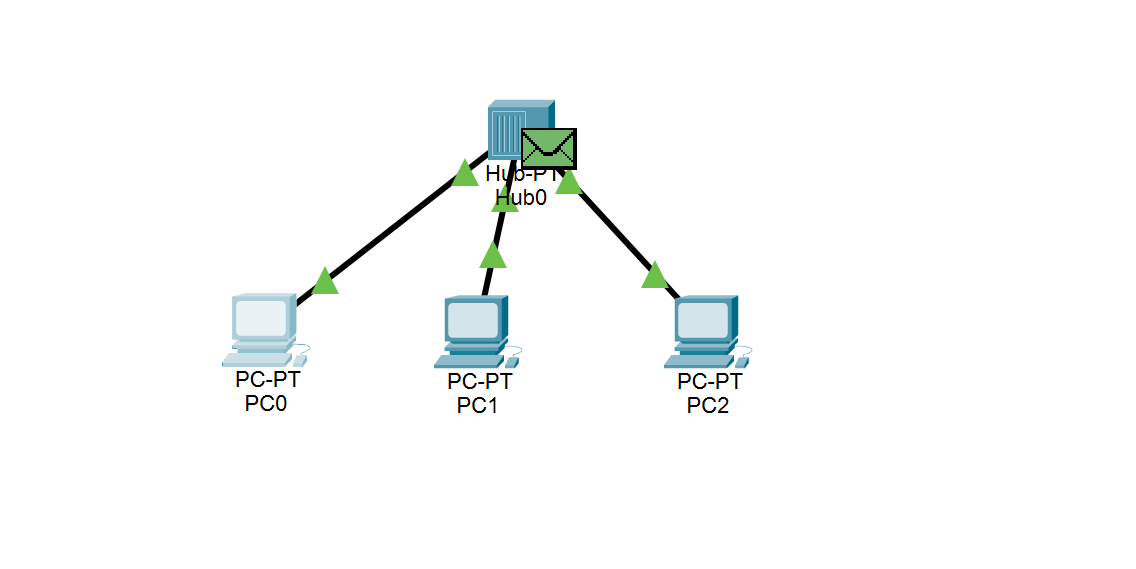
\includegraphics[width=0.78\textwidth]{figure/共享式以太网组网/单集线器/网络拓扑.png}
    \caption{单集线器共享式以太网：PC0、PC1、PC2 连接 Hub0。}
    \label{fig:hub1-topo}
\end{figure}

主机使用静态地址。图~\ref{fig:hub1-ip} 是其中一台的配置，IPv4 为 $192.168.0.1$，掩码 $255.255.255.0$。这就是仿真软件提供的简化配置：在图形界面填写地址，不必进入命令行。

\begin{figure}[htbp]
    \centering
    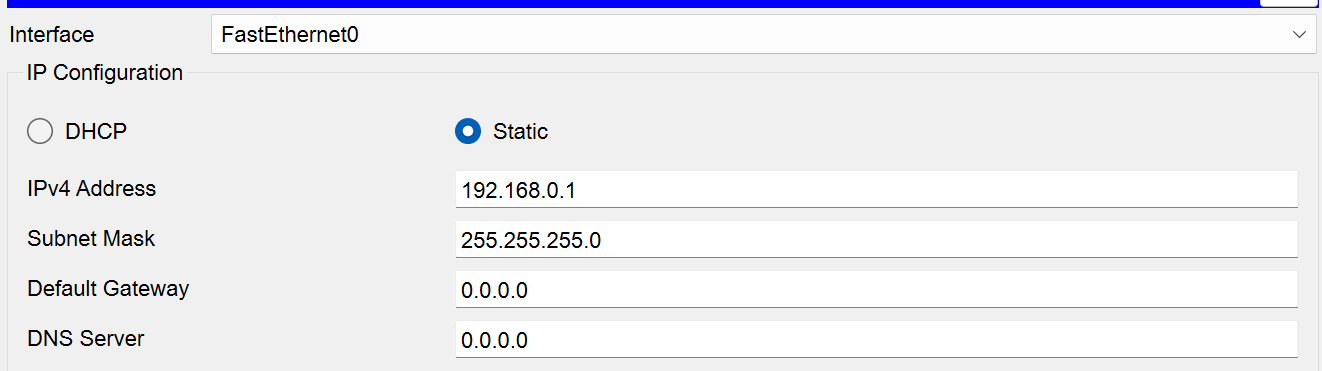
\includegraphics[width=0.92\textwidth]{figure/共享式以太网组网/单集线器/ipconfig.png}
    \caption{单集线器网络中一台主机的 IP 配置。}
    \label{fig:hub1-ip}
\end{figure}

从该网段另一台主机 \texttt{ping} $192.168.0.2$，结果见图~\ref{fig:hub1-ping}。四次探测收到三次应答，丢包率 $25\%$。第一次是 Request timed out，后面三次的往返时间分别为 $8\,\mathrm{ms}$、$4\,\mathrm{ms}$、$4\,\mathrm{ms}$，TTL 均为 128。

\begin{figure}[htbp]
    \centering
    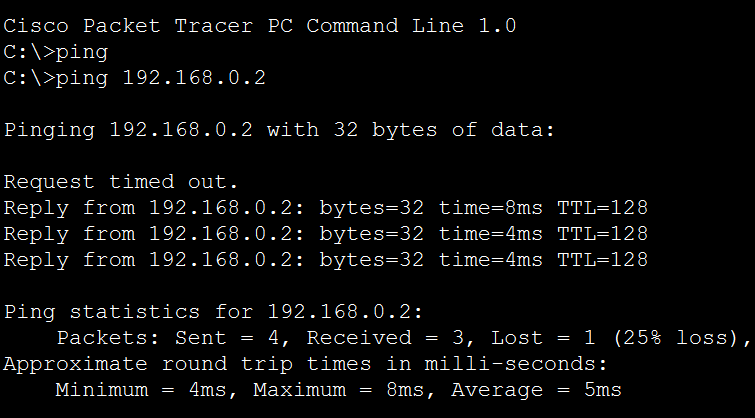
\includegraphics[width=0.92\textwidth]{figure/共享式以太网组网/单集线器/ping.png}
    \caption{PC 命令行 \texttt{ping 192.168.0.2} 的结果。}
    \label{fig:hub1-ping}
\end{figure}

这 $25\%$ 不是链路故障。源主机一开始没有对方的 MAC，第一包要等 ARP 解析，仿真里这次等待记成超时；ARP 完成后，同一条命令里的后三包都得到了 ICMP 应答。TTL 仍是 128，路径上没有路由器。三台主机同处一个网段、一个广播域，所以可以互通。

\subsection{单集线器上的帧传递}
把工作区改到模拟模式，由 PC0 发出报文。图~\ref{fig:hub1-sim} 的事件列表在 $8.022\,\mathrm{s}$ 记录到 PC0，紧接着 $8.023\,\mathrm{s}$ 出现两条 Hub0 事件，工作区里也同时出现两个信封，分别朝 PC1 和 PC2 方向复制。

\begin{figure}[htbp]
    \centering
    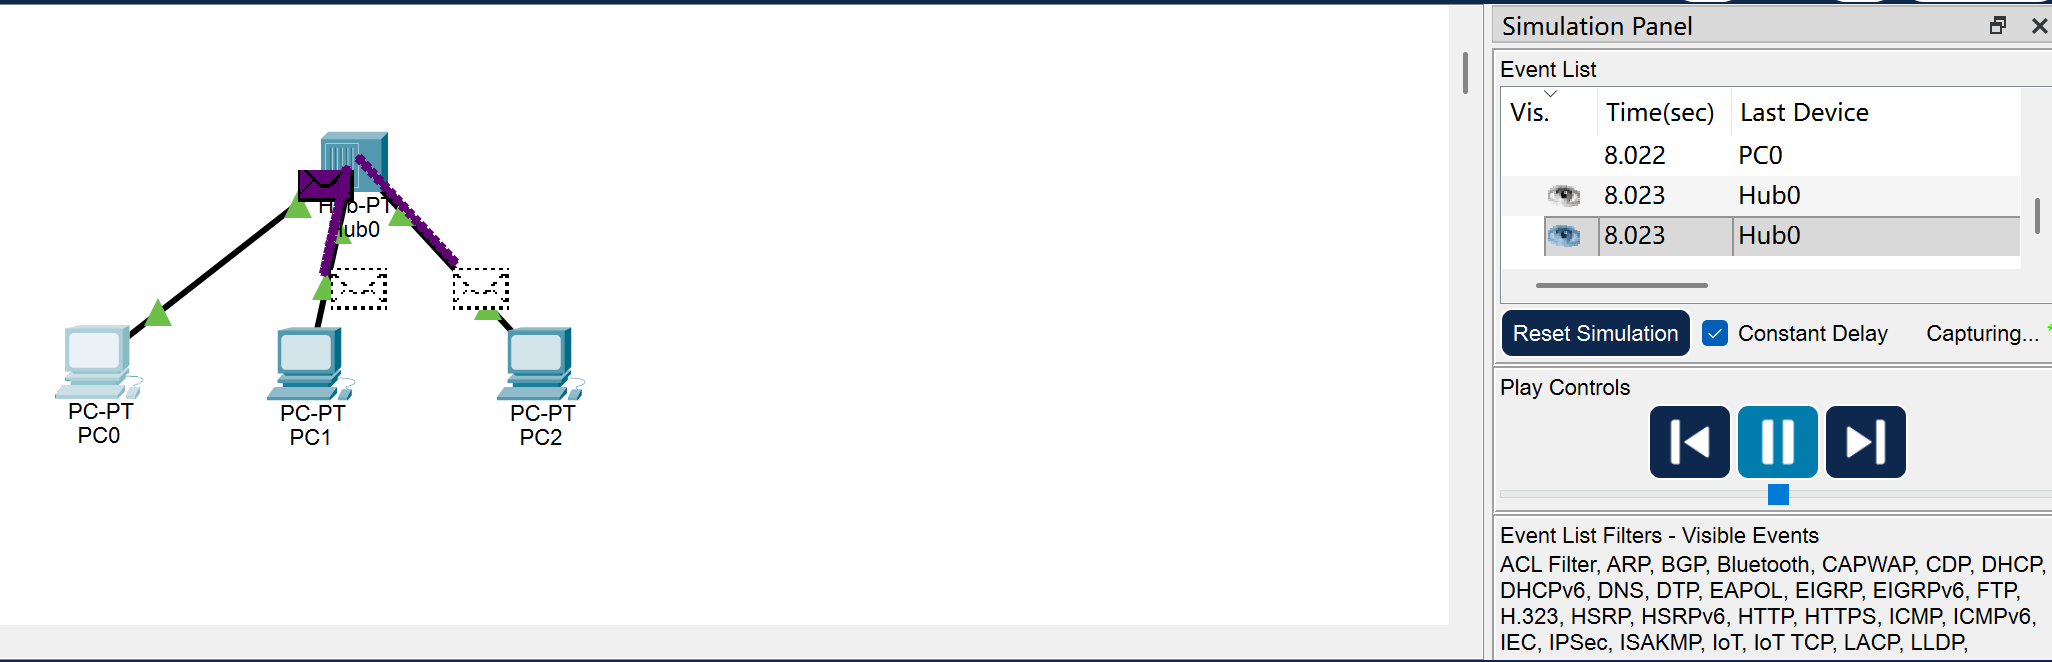
\includegraphics[width=\textwidth]{figure/共享式以太网组网/单集线器/连通性测试.png}
    \caption{模拟模式：Hub0 把 PC0 发出的帧同时复制到另外两个端口。}
    \label{fig:hub1-sim}
\end{figure}

集线器工作在物理层，入端口收到比特流后向其余端口再生，不查看目的 MAC。因此单播帧在介质上的到达范围与广播相同。不是目的主机的网卡会在本机丢弃该帧，但带宽和冲突域已经被占用。Hub0 与三台主机构成一个冲突域，也构成一个广播域。

\subsection{多集线器组网}
Hub0 下接 PC0、PC1、PC2，Hub1 下接 PC3、PC4、PC5，两台集线器级联，见图~\ref{fig:hub2-topo}。

\begin{figure}[htbp]
    \centering
    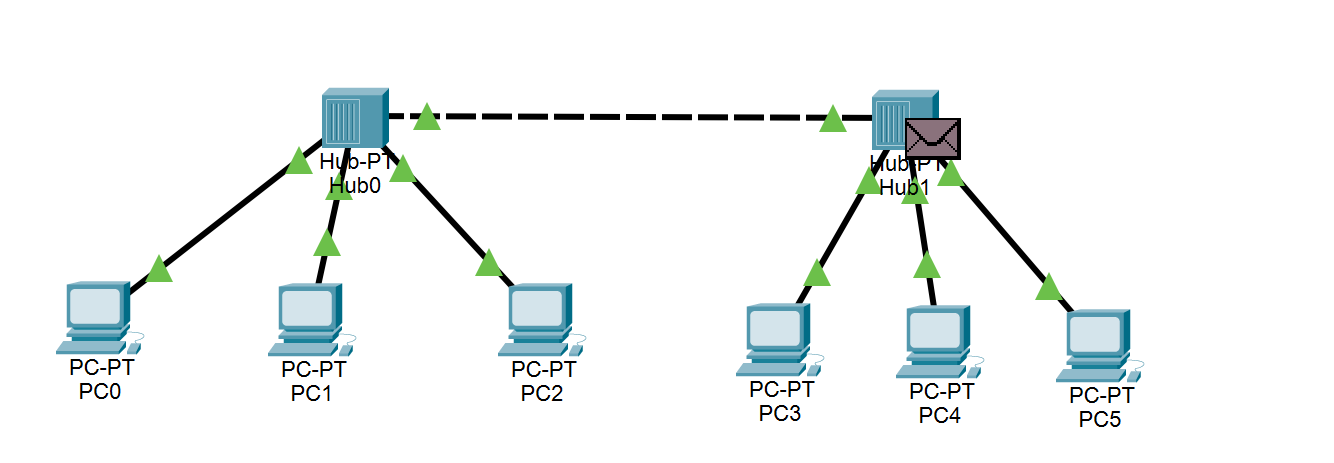
\includegraphics[width=\textwidth]{figure/共享式以太网组网/多集线器/网络拓扑.png}
    \caption{两台集线器级联。六台主机仍在同一共享介质上。}
    \label{fig:hub2-topo}
\end{figure}

图~\ref{fig:hub2-ip} 给出其中一台主机的地址 $192.168.0.6/24$，网关仍为空。对这个地址做 \texttt{ping}，见图~\ref{fig:hub2-ping}：第一包同样超时，随后收到应答，时延 $12\,\mathrm{ms}$，TTL 为 128。时延高于单集线器时的 $4$--$8\,\mathrm{ms}$，因为帧要多穿过一台集线器；TTL 没有减少，说明级联没有加入三层设备。

\begin{figure}[htbp]
    \centering
    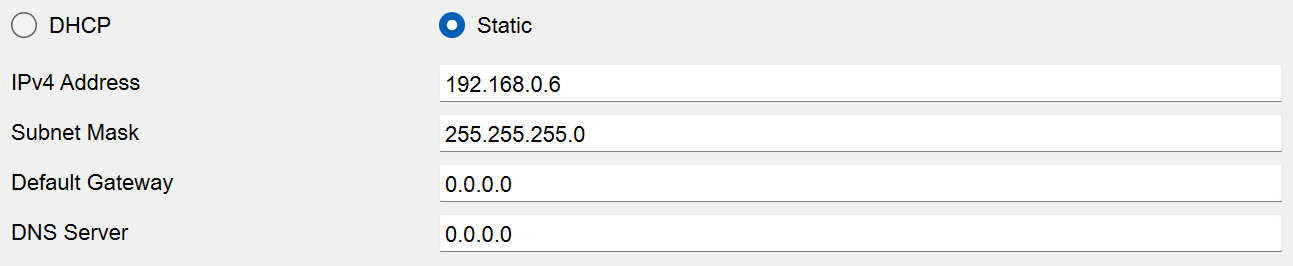
\includegraphics[width=0.82\textwidth]{figure/共享式以太网组网/多集线器/ipconfig.png}
    \caption{多集线器网络中地址为 $192.168.0.6$ 的主机。}
    \label{fig:hub2-ip}
\end{figure}

\begin{figure}[htbp]
    \centering
    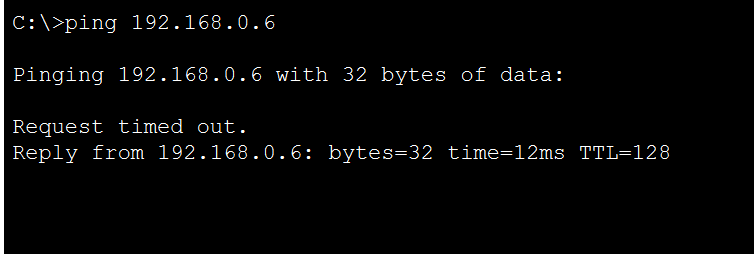
\includegraphics[width=0.88\textwidth]{figure/共享式以太网组网/多集线器/ping.png}
    \caption{跨集线器 \texttt{ping 192.168.0.6}：首包超时后收到应答。}
    \label{fig:hub2-ping}
\end{figure}

模拟模式的一瞬见图~\ref{fig:hub2-sim}。帧经过级联到达 Hub0 后被复制到 PC0、PC1、PC2。PC0 接受该 PDU，显示为成功；PC1 与 PC2 的目的 MAC 不匹配，显示为失败。级联只是把物理介质接长，并没有按地址过滤。六台主机仍然共享一个冲突域和一个广播域，任意同网段主机都能互通，同时任一主机发送都会占用整条级联链。

\begin{figure}[htbp]
    \centering
    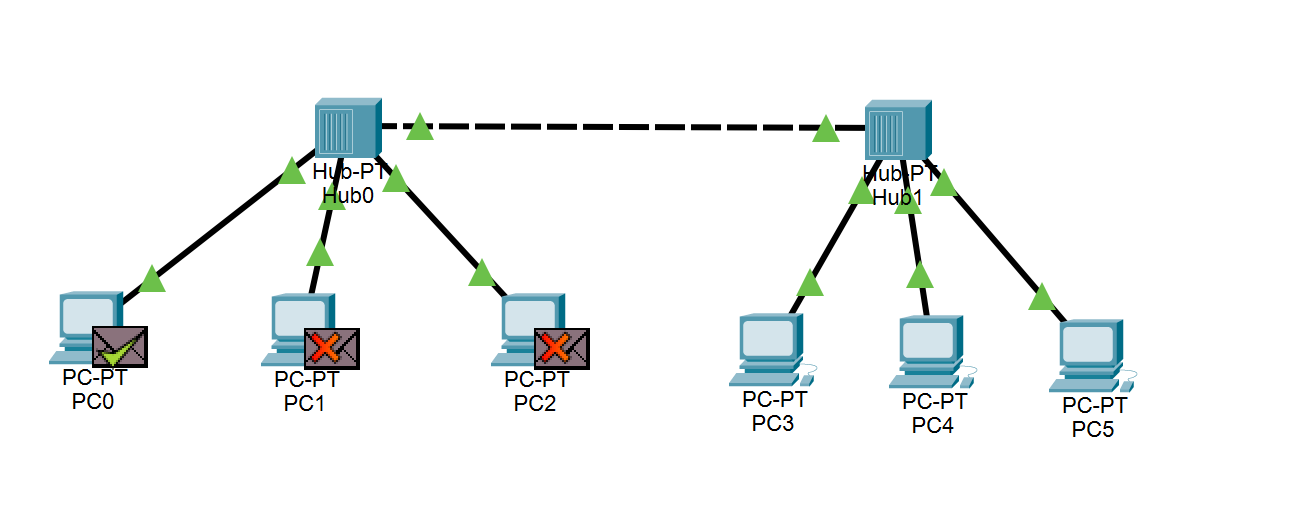
\includegraphics[width=\textwidth]{figure/共享式以太网组网/多集线器/连通性测试.png}
    \caption{多集线器模拟：目的主机 PC0 接受帧，同一集线器上的 PC1、PC2 丢弃帧。}
    \label{fig:hub2-sim}
\end{figure}

\section{交换式以太网与 VLAN}
\subsection{单交换机组网}
用一台 2960-24TT 替换集线器，见图~\ref{fig:sw-topo}。PC6、PC7、PC8 经直通线接入，PC9 经 Console 线接到交换机，供终端配置使用。用户数据不会出现在这根青色线上。

\begin{figure}[htbp]
    \centering
    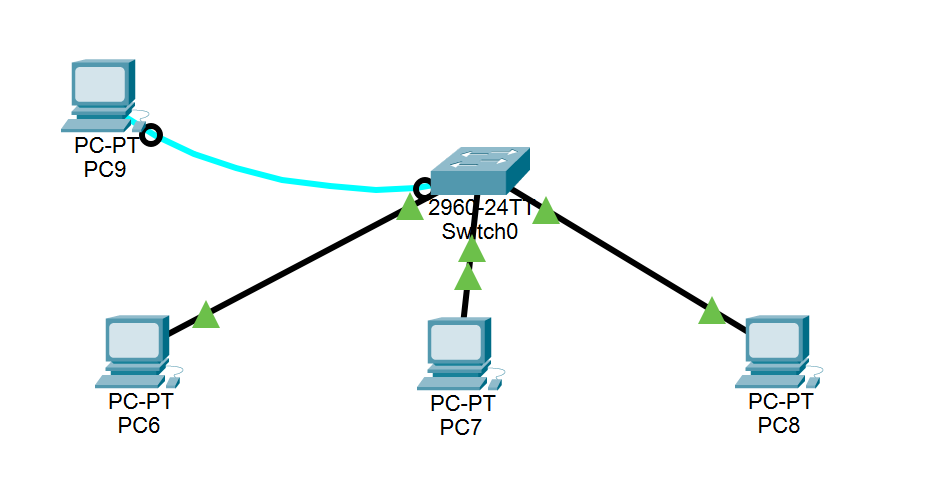
\includegraphics[width=0.82\textwidth]{figure/交换式以太网组网/单交换机/拓扑结构.png}
    \caption{单交换机以太网。PC9 与 Switch0 之间是 Console 线。}
    \label{fig:sw-topo}
\end{figure}

\texttt{ping 192.168.0.4} 的三次可见应答都成功，时延为 $8\,\mathrm{ms}$、$4\,\mathrm{ms}$、$4\,\mathrm{ms}$，TTL 为 128，见图~\ref{fig:sw-ping}。这次没有出现首包超时，说明 ARP 缓存里已经有目的 MAC。连通性与集线器网络相同，差别在转发范围。

\begin{figure}[htbp]
    \centering
    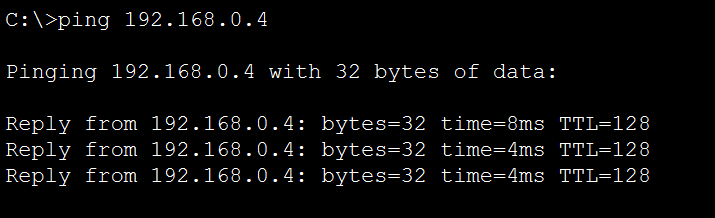
\includegraphics[width=0.9\textwidth]{figure/交换式以太网组网/单交换机/ping.png}
    \caption{单交换机网络中 \texttt{ping 192.168.0.4} 的应答。}
    \label{fig:sw-ping}
\end{figure}

图~\ref{fig:sw-sim} 是学习完成后的模拟结果：信封只出现在 PC6 上，PC7 和 PC8 的链路上没有这份单播。交换机已经知道目的 MAC 位于哪一个端口，不再向其余接入端口泛洪。

\begin{figure}[htbp]
    \centering
    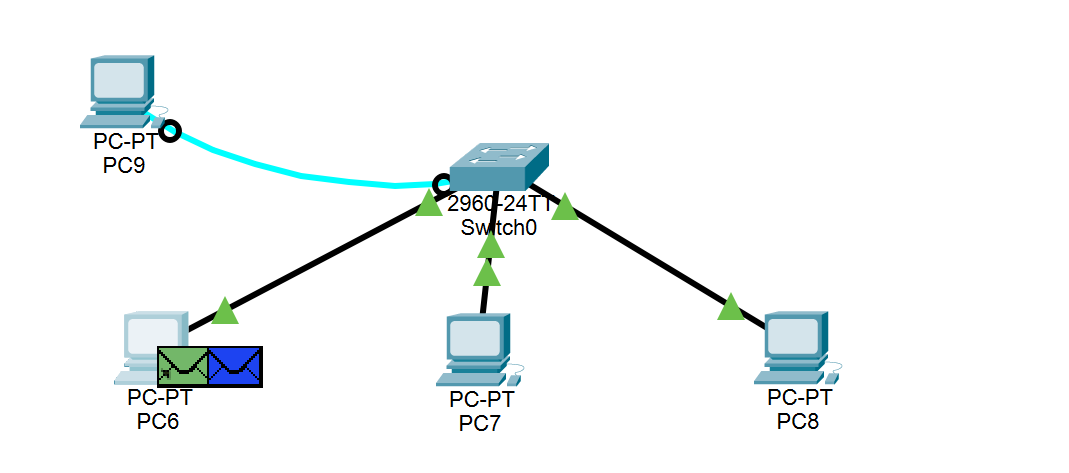
\includegraphics[width=0.82\textwidth]{figure/交换式以太网组网/单交换机/连通性测试.png}
    \caption{MAC 地址学习之后，单播帧只到达目的主机 PC6。}
    \label{fig:sw-sim}
\end{figure}

\subsection{终端方式查看地址表}
通过 Console 进入交换机 CLI，执行 \texttt{show mac address-table}，见图~\ref{fig:mac}。表中只有通信过的两条动态表项，都在 VLAN 1：

\begin{itemize}[leftmargin=2em]
    \item \texttt{0002.1734.0dcd} $\rightarrow$ FastEthernet0/2；
    \item \texttt{0030.f247.0cba} $\rightarrow$ FastEthernet0/3。
\end{itemize}

\begin{figure}[htbp]
    \centering
    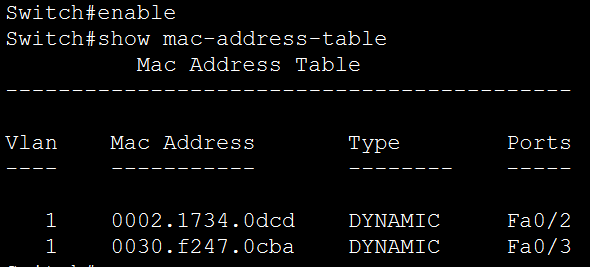
\includegraphics[width=0.82\textwidth]{figure/交换式以太网组网/单交换机/mac-address-table.png}
    \caption{终端中的 MAC 地址表。只记录了已经发出过帧的主机。}
    \label{fig:mac}
\end{figure}

对照两台主机的网卡配置，可以确认表项从何而来。图~\ref{fig:mac1} 中 MAC 为 \texttt{0002.1734.0DCD} 的主机地址是 $192.168.0.3$，对应 Fa0/2。图~\ref{fig:mac2} 中 MAC 为 \texttt{0030.F247.0CBA} 的主机地址是 $192.168.0.4$，对应 Fa0/3。交换机按入端口的源 MAC 学习，没有发过帧的主机不会出现在表里，所以截图中看不到第三台接入主机。每个接入端口是一个冲突域；在尚未划分 VLAN 时，这些端口仍属于同一个广播域 VLAN 1。

\begin{figure}[htbp]
    \centering
    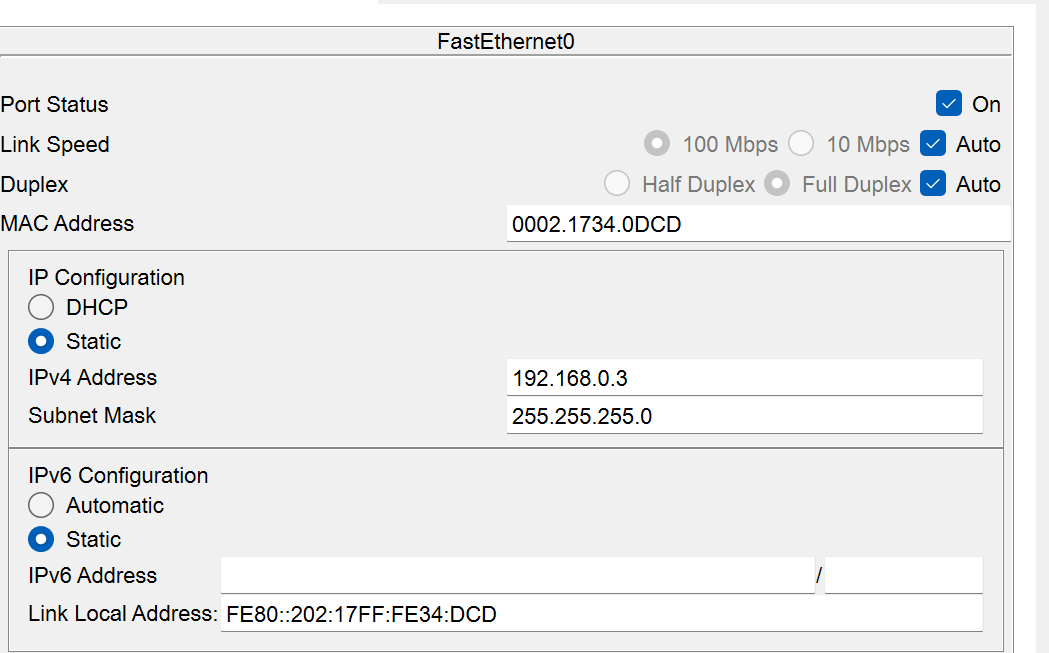
\includegraphics[width=0.72\textwidth]{figure/交换式以太网组网/单交换机/mac-address1.png}
    \caption{$192.168.0.3$ 的网卡地址，与 Fa0/2 的表项一致。}
    \label{fig:mac1}
\end{figure}

\begin{figure}[htbp]
    \centering
    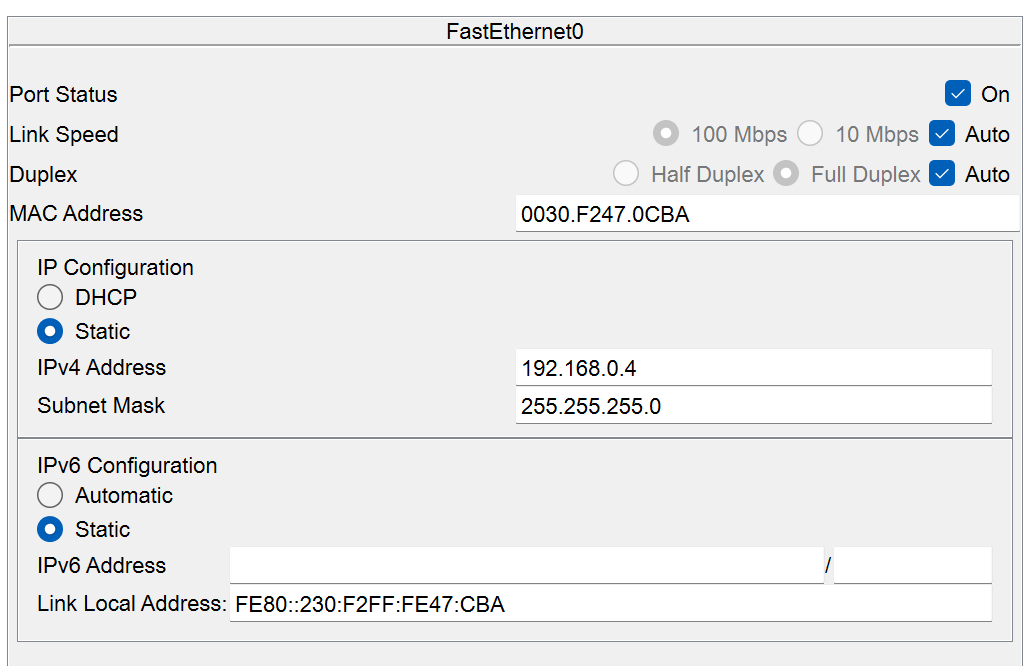
\includegraphics[width=0.72\textwidth]{figure/交换式以太网组网/单交换机/mac-address2.png}
    \caption{$192.168.0.4$ 的网卡地址，与 Fa0/3 的表项一致。}
    \label{fig:mac2}
\end{figure}

\subsection{简化配置与单交换机 VLAN}
VLAN 没有逐条输入 IOS，而是用 Config 选项卡完成，这是 Packet Tracer 的简化配置。图~\ref{fig:vlan} 在 VLAN Database 中新增 VLAN 2，名称为 \texttt{test}。默认 VLAN 1 以及 1002--1005 是交换机自带的，不能当作本次划分的用户 VLAN。

\begin{figure}[htbp]
    \centering
    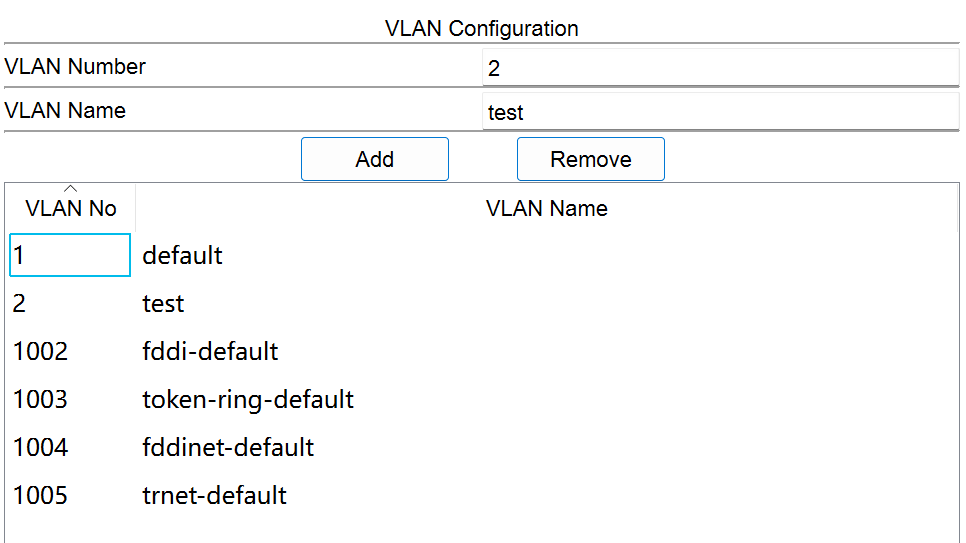
\includegraphics[width=0.78\textwidth]{figure/交换式以太网组网/单交换机/VLAN.png}
    \caption{图形界面创建 VLAN 2，名称为 test。}
    \label{fig:vlan}
\end{figure}

图~\ref{fig:vlan-set} 把 FastEthernet0/1 的模式设为 Access，VLAN 选 2。Access 端口发出的帧不带 802.1Q 标签，进入该端口的帧全部归入 VLAN 2。其余主机端口保持在 VLAN 1。图形界面写入的仍是运行配置，等价的命令是 \texttt{switchport mode access} 与 \texttt{switchport access vlan 2}。

\begin{figure}[htbp]
    \centering
    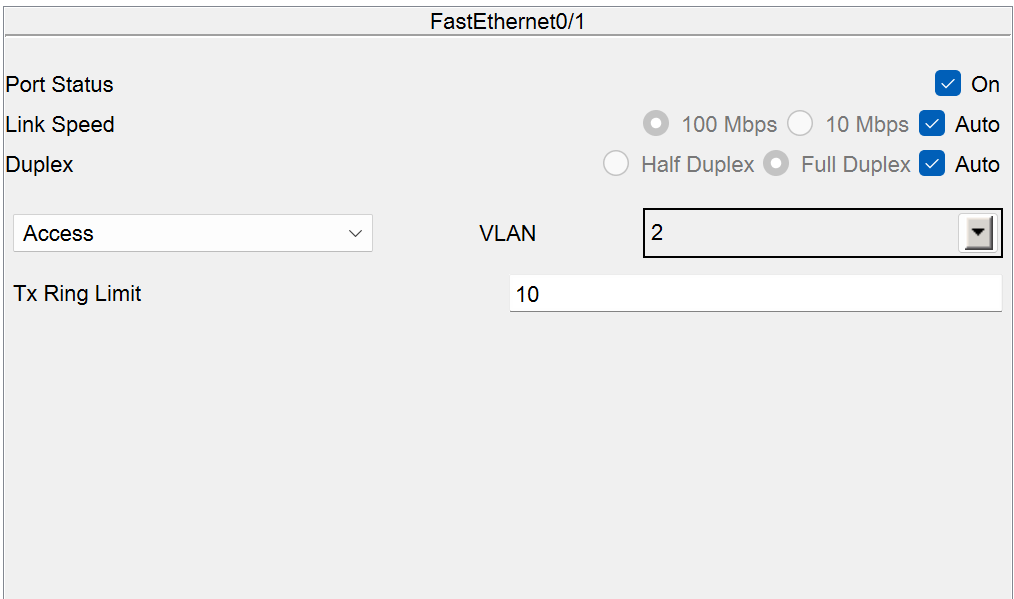
\includegraphics[width=0.82\textwidth]{figure/交换式以太网组网/单交换机/VLAN-set.png}
    \caption{FastEthernet0/1 设为 Access，划入 VLAN 2。}
    \label{fig:vlan-set}
\end{figure}

隔离结果见图~\ref{fig:vlan-iso}。PC6 一侧的端口离开 VLAN 1 之后，发往该主机的 PDU 失败，交换机对应端口上也出现了告警标记。同一 VLAN 内的主机仍可按上一节的方式互通；PC6 与留在 VLAN 1 的主机之间，ARP 广播到不了对端，\texttt{ping} 得不到应答。交换机不在 VLAN 之间转发二层帧，本实验又没有路由器，所以不同 VLAN 不能通信。

\begin{figure}[htbp]
    \centering
    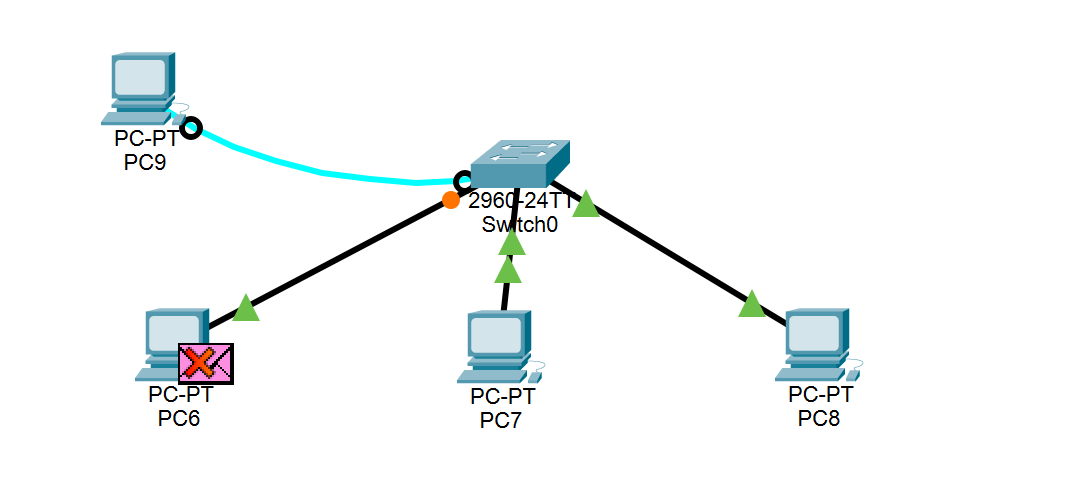
\includegraphics[width=0.82\textwidth]{figure/交换式以太网组网/单交换机/VLAN-isolation.png}
    \caption{PC6 被划入另一 VLAN 后，发往该主机的 PDU 失败。}
    \label{fig:vlan-iso}
\end{figure}

\subsection{混合网络与跨交换机 VLAN}
拓扑见图~\ref{fig:hy-topo}。Switch1 接入 PC12、PC13，并通过 Hub2 接入 PC14；Switch2 通过 Hub3 接入 PC15、PC16、PC17。PC10、PC11 分别用 Console 线管理两台交换机。两台交换机之间是虚线所示的互联链路。Hub2、Hub3 接在接入端口上：集线器不能识别标签，同一台集线器上的主机只能属于一个 VLAN，它们还共享该接入端口所在的冲突域。

\begin{figure}[htbp]
    \centering
    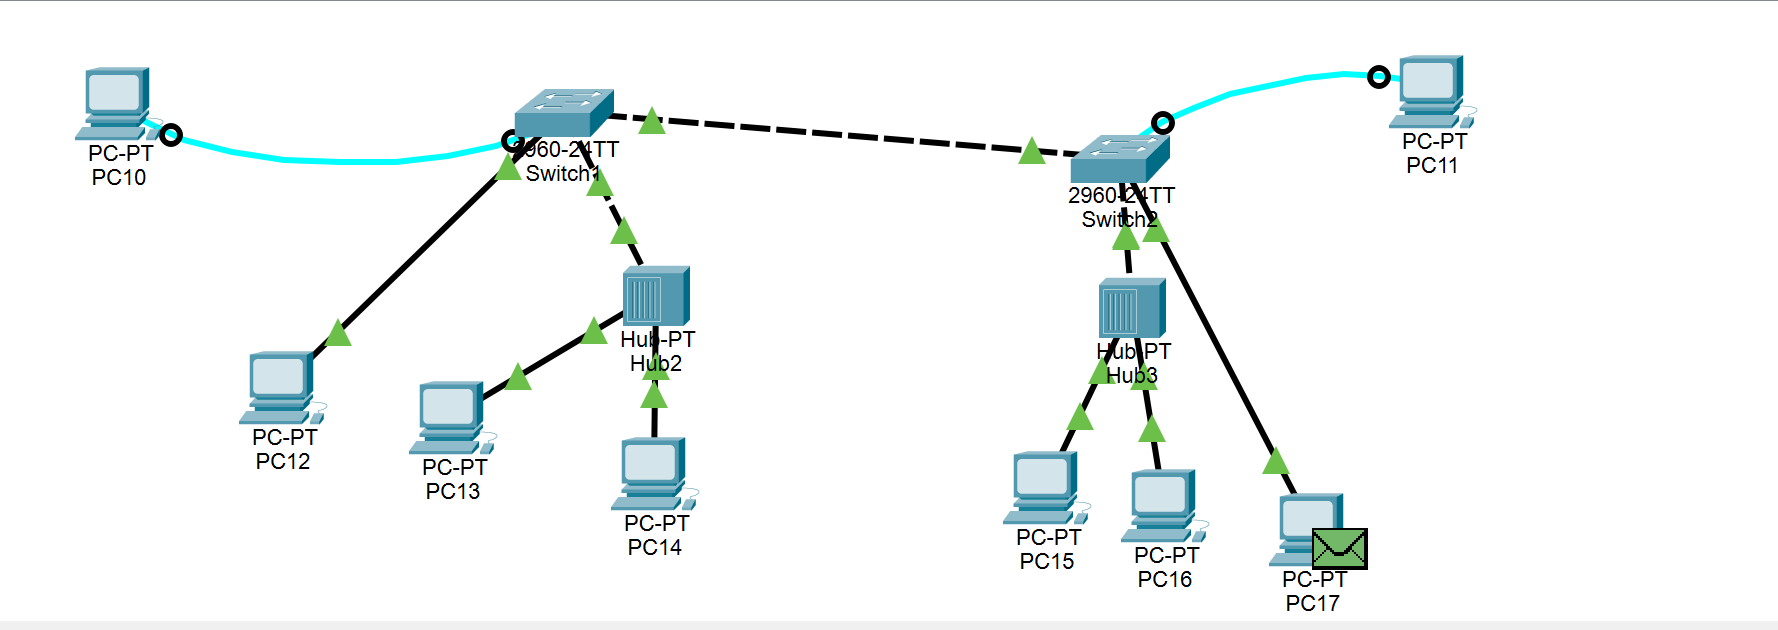
\includegraphics[width=\textwidth]{figure/交换式以太网组网/多交换机/拓扑结构.png}
    \caption{两台交换机、两台集线器的混合网络。青色线为 Console，虚线为交换机互联。}
    \label{fig:hy-topo}
\end{figure}

两侧都需要相同的 VLAN 编号，否则对端无法识别标签。图~\ref{fig:hy-vlan} 在已有 VLAN 2（test）之外增加 VLAN 3，名称为 \texttt{vip}。图~\ref{fig:trunk} 把互联端口 FastEthernet0/1 的模式改为 Trunk，VLAN 下拉框仍是 1，表示本征 VLAN 保持默认值。Trunk 可以同时承载 VLAN 2 和 VLAN 3，数据帧带 802.1Q 标签，本征 VLAN 的帧不带标签。

\begin{figure}[htbp]
    \centering
    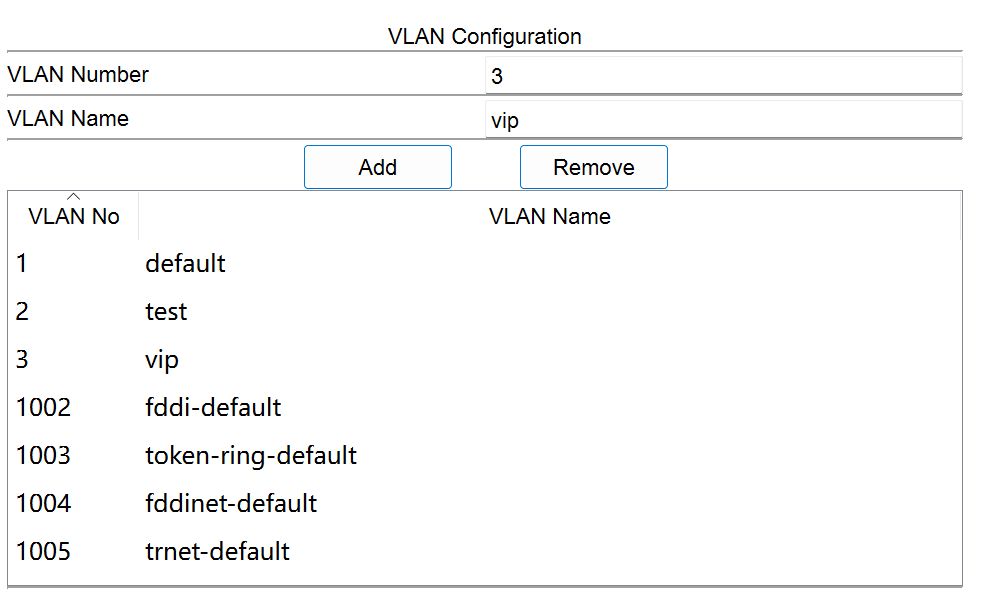
\includegraphics[width=0.78\textwidth]{figure/交换式以太网组网/多交换机/VLAN.png}
    \caption{混合网络中的 VLAN：1 为默认，2 为 test，3 为 vip。}
    \label{fig:hy-vlan}
\end{figure}

\begin{figure}[htbp]
    \centering
    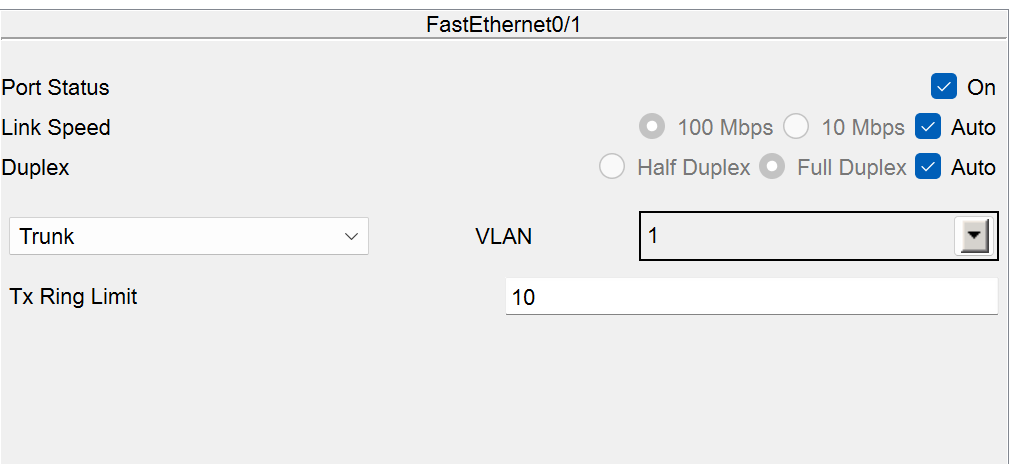
\includegraphics[width=0.82\textwidth]{figure/交换式以太网组网/多交换机/Trunk.png}
    \caption{交换机互联端口 FastEthernet0/1 设为 Trunk。}
    \label{fig:trunk}
\end{figure}

同一 VLAN 的测试见图~\ref{fig:hy-ping} 与图~\ref{fig:hy-sim}。\texttt{ping 192.168.2.42} 收到应答，时延 $12\,\mathrm{ms}$，TTL 为 128。这个时延与多集线器跨设备时的 $12\,\mathrm{ms}$ 相同，高于单交换机直连时的 $4\,\mathrm{ms}$，符合「帧经过 Trunk，必要时还经过集线器」的路径。模拟画面里成功标记只出现在 PC12，没有扩散到 PC13 或 Hub2。交换机在 VLAN 内部按 MAC 表单播转发；集线器只在帧已经被送到它所接的那个接入端口时才会复制。

\begin{figure}[htbp]
    \centering
    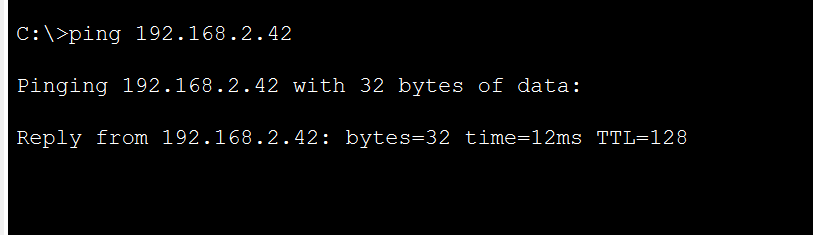
\includegraphics[width=0.88\textwidth]{figure/交换式以太网组网/多交换机/ping.png}
    \caption{跨交换机 \texttt{ping 192.168.2.42} 得到应答。}
    \label{fig:hy-ping}
\end{figure}

\begin{figure}[htbp]
    \centering
    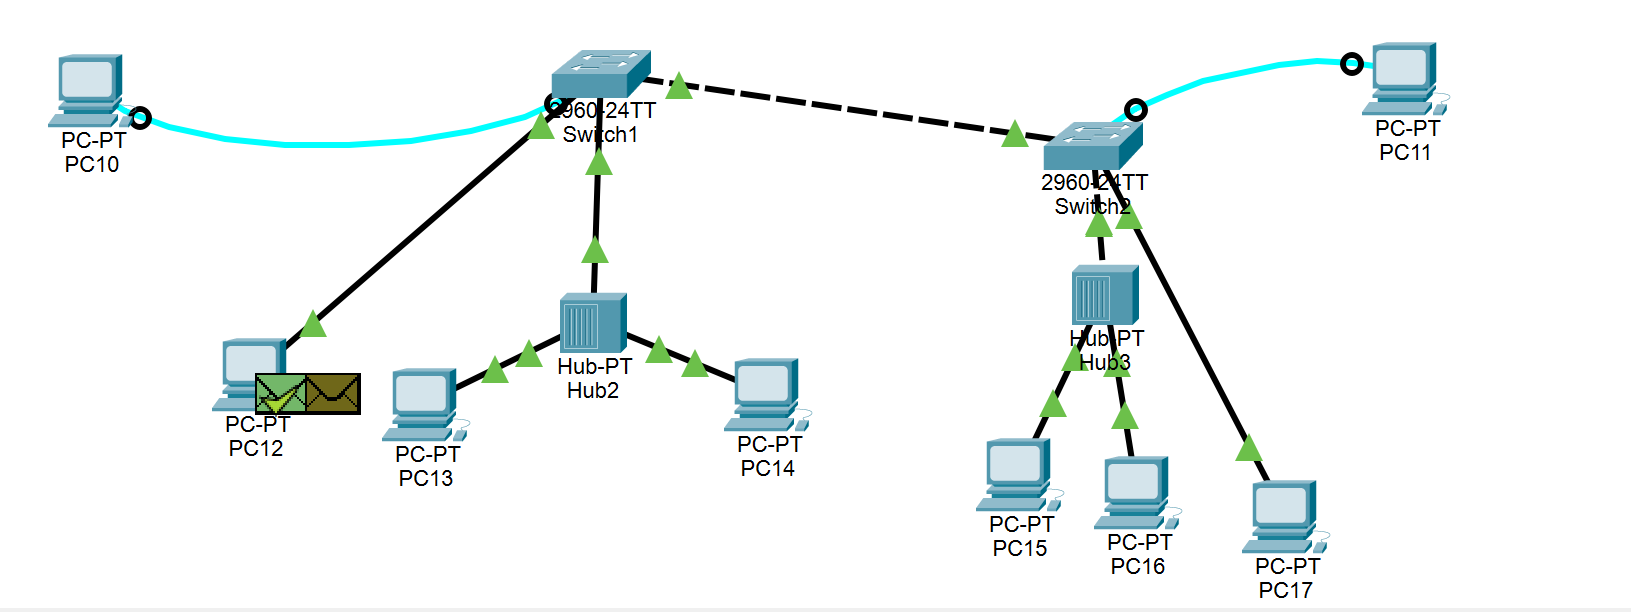
\includegraphics[width=\textwidth]{figure/交换式以太网组网/多交换机/连通性测试.png}
    \caption{同一 VLAN 的 PDU 被送到 PC12，没有在 Switch1 的其他接入主机上泛洪。}
    \label{fig:hy-sim}
\end{figure}

不同 VLAN 的测试见图~\ref{fig:hy-iso}。\texttt{ping 192.168.0.37} 四次都是 Request timed out，丢包率 $100\%$。命令行给出的是超时而不是 Destination host unreachable，说明源主机把 $192.168.0.37$ 看成同一网段上的地址，报文已经发出，失败发生在得不到 ARP 或 ICMP 应答。Trunk 只是让同一个 VLAN 跨过两台交换机，不会把 VLAN 2 和 VLAN 3 接起来。目的主机若在另一个 VLAN，广播到不了它，即使两台主机都接在这张混合拓扑里也不通。

\begin{figure}[htbp]
    \centering
    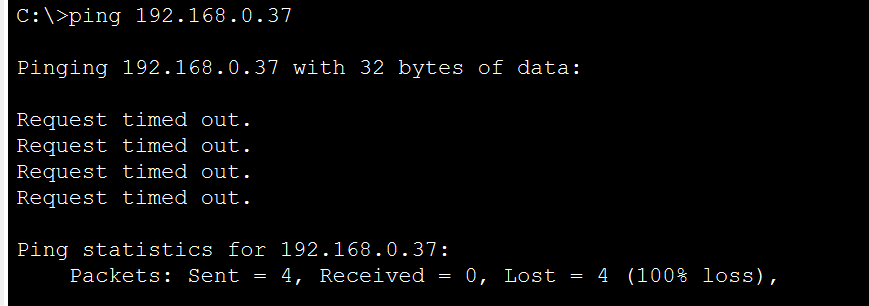
\includegraphics[width=0.9\textwidth]{figure/交换式以太网组网/多交换机/isolation.png}
    \caption{跨 VLAN \texttt{ping 192.168.0.37}：四次超时，丢包率 $100\%$。}
    \label{fig:hy-iso}
\end{figure}

\subsection{几种拓扑中的传递过程}
把四张模拟截图放在一起，可以看到设备每增加一种能力，帧的到达范围就缩小一档。

\begin{enumerate}[leftmargin=2em]
    \item 单集线器（图~\ref{fig:hub1-sim}）：PC0 发出一帧，Hub0 在同一时刻复制出两份。目的 MAC 是否已知不影响复制范围。
    \item 多集线器（图~\ref{fig:hub2-sim}）：级联后的集线器继续复制。目的主机接受，同网段的其余主机丢弃。丢弃发生在网卡，不发生在集线器。
    \item 单交换机（图~\ref{fig:sw-sim}）：MAC 表记下源地址与端口后，单播只从对应端口送出。图~\ref{fig:mac} 里 Fa0/2、Fa0/3 各有一条表项，就是这个学习结果。广播和未知单播仍会在同一 VLAN 内泛洪，所以交换机分开的是冲突域，不是广播域。
    \item 混合网络（图~\ref{fig:hy-sim}、图~\ref{fig:hy-iso}）：同一 VLAN 的单播可以穿过 Trunk 到达 PC12；另一个 VLAN 中的 $192.168.0.37$ 没有任何应答。Hub2、Hub3 只扩展各自接入端口的冲突域，不能把两个 VLAN 合成一个广播域。
\end{enumerate}

\section{现象归纳}
表~\ref{tab:summary} 按截图中的现象比较四种拓扑。共享式以太网的「能通」伴随全端口复制；交换式以太网的「能通」在地址学习后只占用目的端口；VLAN 则使另一部分同拓扑主机变为超时。

\begin{table}[htbp]
\centering
\caption{四种拓扑的观察结果}
\label{tab:summary}
\begin{tabular}{lll}
\toprule
拓扑 & 连通性 & 模拟模式下帧的范围 \\
\midrule
单集线器 & \texttt{.2} 后三包成功 & Hub0 复制到全部其他端口 \\
多集线器级联 & \texttt{.6} 超时后成功 & 非目的主机丢弃，集线器仍复制 \\
单交换机 & \texttt{.4} 应答成功 & 学习后只到达 PC6 \\
混合网络，同一 VLAN & \texttt{192.168.2.42} 成功 & 只标记在目的主机 PC12 \\
混合网络，不同 VLAN & \texttt{192.168.0.37} 全部超时 & 报文不能进入另一 VLAN \\
\bottomrule
\end{tabular}
\end{table}

\section{结论}
\begin{enumerate}[leftmargin=2em]
    \item 单集线器网络中，\texttt{ping 192.168.0.2} 的第一包因 ARP 超时，后三包成功。模拟模式里 Hub0 把一帧复制成两份，三台主机属于同一个冲突域。
    \item 两台集线器级联后，\texttt{ping 192.168.0.6} 仍然成功，时延升到 $12\,\mathrm{ms}$。非目的主机显示失败，只说明网卡丢弃了帧，冲突域并没有被级联拆开。
    \item 单台 2960 上，\texttt{ping 192.168.0.4} 成功。终端中的 MAC 表把 $192.168.0.3$ 记在 Fa0/2、把 $192.168.0.4$ 记在 Fa0/3，之后单播只出现在目的主机 PC6 上。
    \item 用图形界面建立 VLAN 2（test），并把 Fa0/1 划为该 VLAN 的 Access 端口后，PC6 与其余主机不再互通。简化配置与 CLI 写入的是同一份端口模式。
    \item 混合网络中，两台交换机具有 VLAN 2 和 VLAN 3，互联端口为 Trunk。同一 VLAN 的 $192.168.2.42$ 可以跨交换机应答；不同 VLAN 的 $192.168.0.37$ 四次超时。集线器只扩展某一个 VLAN 的接入冲突域。
\end{enumerate}

\end{document}
